\chapter{Background} \label{chap:background}

\section{Organic Semiconductors}

%When atoms bond together, molecular orbital are defined by the linear combination of atomic orbitals, however the symmetry shown on some complex structures are not explained by a simple linear combination, instead hybrid atomic orbitals are formed. This mathematical process is called \textbf{hybridization}.
Unlike inorganic semiconductors, organic semiconductors are lightweight, easy to chemically tune, mechanical flexible, and offer low-cost and low-temperature processing. All of these characteristics are responsible for the increased attention to this type of materials in the field of organic electronics. 

%\subsection{Conjugated polymers}
%\subsection{Small molecules}

\subsection{Electronic Structure and Transport} 

Organic semiconductors are $\pi$-conjugated molecules that comprise mostly carbon and hydrogen atoms, with alternating multiple (sp$^{2}$ hybridization) and single (sp hybridization) bonds. The wavefunction of the sp$^{2}$ orbitals overlap so that electrons can be delocalized.
%This configuration exhibit $p$-orbitals with delocalized electrons. %, charge transport among the length of these polymers is caused by the alternation of these bonds, describing a resonance structure. 
Based on the size of the conjugated system, organic semiconductors can be divided into conjugated polymers and small molecules. The latter has the advantage of being ordered and its synthesis allows to obtain high purity material \cite{alcacerElectronicStructureOrganic2018}.

\begin{figure}[h]
  \centering
  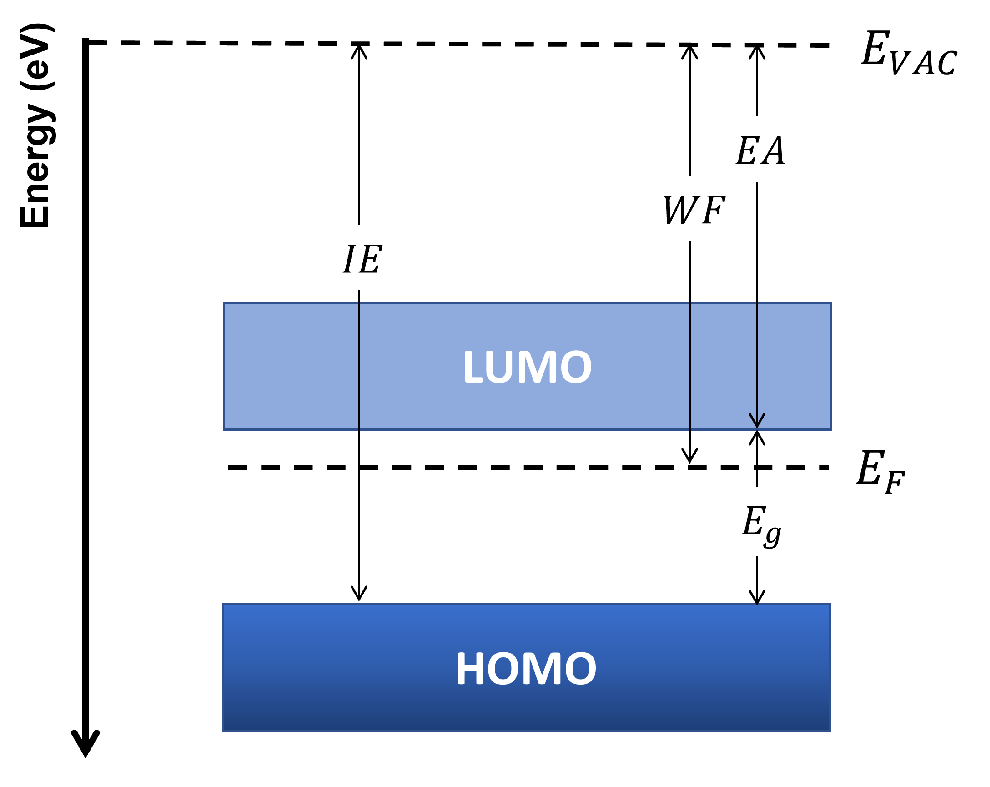
\includegraphics[width=6cm]{Images/pdf/ediagram.pdf}
  \caption[Energy level diagram of organic semiconductors]{Energy level diagram of an n-type doped organic semiconductor.}
  \label{fig:ediag}
\end{figure}

The energy structure of organic semiconductors comprises a highest occupied molecular orbital (HOMO) and a lowest unoccupied molecular orbital (LUMO), that are analogous to the valence and conduction %bands
states, respectively, from inorganic semiconductors. The difference between both energy levels corresponds to the energy gap (E$_{g}$) of the material, as represented in Figure \ref{fig:ediag}. We could also defined i) the Fermi level (E$_{F}$) using the material work function (WF), ii) the ionization energy (IE, also referred as ionization potential, IP), using the HOMO energy, and iii) the electron affinity (EA), using the LUMO energy.

%\subsubsection{Conjugated polymers}
%Semiconducting properties of conjugated polymers built by alternating electron donor and acceptor moieties \cite{mattElectronicStructureMorphology2021}, 
%Since inorganic semiconductors' band models does not take into consideration the Coulomb and exchange electron-electron interaction, which play a major role in organic semiconductors, it is necessary to add new theoretical approaches. On one hand, the transport properties are better described in terms of a hopping mechanism and the optoelectronic properties are better described by the molecular orbital picture \cite{alcacerElectronicStructureOrganic2018}. Since the device under study in this work is a transistor and their transport properties in aqueous and quasi-solid environments, the theoretical approach used will be the hopping mechanism.

%Transport properties depend on the details of the band structure, namely the density of states and the band widths

%\subsubsection{Small Molecules}
%Unlike conjugated polymers, the chain size of small molecules have the advantage of being ordered and its synthesis allow to obtain high purity material.

%\subsection{Electronic Transport}

An organic semiconductor material could also be classified depending on whether the ground state is degenerate or non-degenerate. The former describes monomers that are energetically equivalent in the ground state, and in the latter, the opposite happens, commonly seen due to the energy difference of aromatic (benzoid) and quinoid structures \cite{heegerSolitonsConductingPolymers1988a}, as exhibited in Figure \ref{fig:energy}.

\begin{figure}[h]
  \centering
  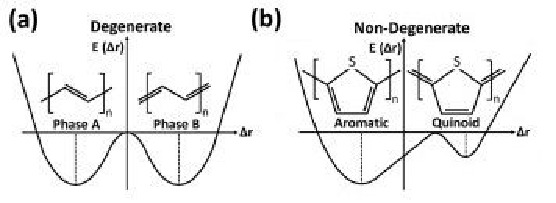
\includegraphics[width=12cm]{Images/pdf/deg_pol.pdf}
  \caption[Degenerate and non-degenerate conjugated polymers]{Potential energy change (electronic plus lattice distortion energy) in a) degenerate and b) non-degenerate ground-state-conjugated polymers. Extracted from reference \cite{heydarigharahcheshmehTextureNanostructuralEngineering2020}.}
  \label{fig:energy}
\end{figure}

%Transport in an organic semiconductor creates changes in the bond-length alternation pattern. Since charge transport come together with a chain distortion, new quasiparticles are defined: solitons in degenerate molecules and polarons in non-degenerate molecules \cite{bredasRoleMobileOrganic1984}.
Transport within an organic semiconductor induces alterations in the bond-length alternation pattern. As charge transport occurs, it is accompanied by chain distortions, leading to the emergence of novel quasiparticles: solitons within degenerate molecules and polarons within non-degenerate molecules \cite{bredasRoleMobileOrganic1984}.

 %Since charge transport come together with a chain distortion, new quasiparticles are defined in transport theory, in a degenerated molecule, the quasiparticles are named solitons, and in a non-degenerated molecule, a bound soliton-antisoliton is formed in the benzoid structures, the pair receive the name of polaron. This pair annihilate in the quinoid structure in between forming a double bond so neutral polarons are not stable \cite{bredasRoleMobileOrganic1984}.

\subsection{Molecular Doping} \label{subsec:moldop}
The basic principles of molecular doping are similar than in inorganic materials. A donor or acceptor entity is added to generate electrons or holes, as shown in Figure \ref{fig:dopscheme}. While n-type dopants donate electrons to the lowest unoccupied molecular orbital (LUMO) states, the p-type dopants extract electrons from the highest occupied molecular orbital (HOMO) states, hence they create holes \cite{lussemDopingOrganicSemiconductors2013}. In other words, the Fermi level E$_{F}$ of the polymer will shift towards the LUMO (or HOMO) level when there is n-type (or p-type) doping. This shift can be measured by spectroscopy techniques such as Ultraviolet Photoelectron Spectroscopy (UPS) at room temperature (RT) \cite{tietzeFermiLevelShift2012}, although a bit limited by the penetration depth of the incoming electrons.

\begin{figure}[h]
  \centering
  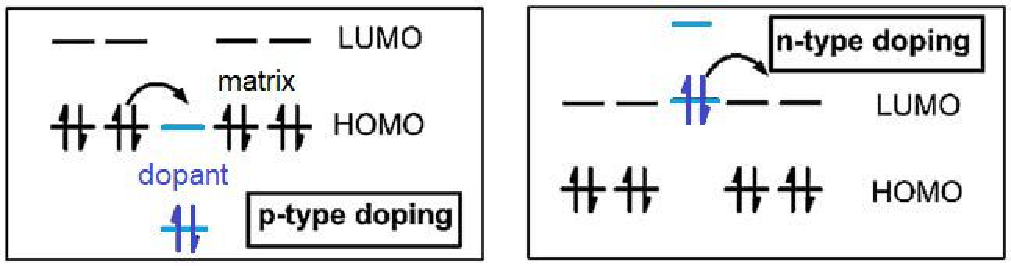
\includegraphics[width=12cm]{Images/pdf/doping.pdf}
  \caption[Scheme of doping processes in organic semiconductors]{Schemes for p-type (left) and n-type (right) doping processes. Extracted from reference \cite{lussemDopingOrganicSemiconductors2013}.}
  \label{fig:dopscheme}
\end{figure}

When doping occurs, %charged solitons come as outcome in a degenerated molecules. In a non-degenerated, our main focus in this work, 
the formation of a new quasiparticle named bipolaron occurs. For instance, if p-type dopant is introduced to a degenerate molecule (Figure \ref{fig:bipol}), electrons are removed from double bonds, if we focus on just one event, while one carbon is left positively charged, the adjacent has an unpaired electron. This unpaired electron shifts down the polymer chain until reaching another unpaired electron from a separated doping event, together they form a double bond, leaving aside two charged polarons: a bipolaron, which unlike a single polaron, it is stable \cite{bredasPolaronsBipolaronsSolitons1985}. %Although, a nice simplification, in a degenerated molecule is not realistic, but usually

\begin{figure}[h]
  \centering
  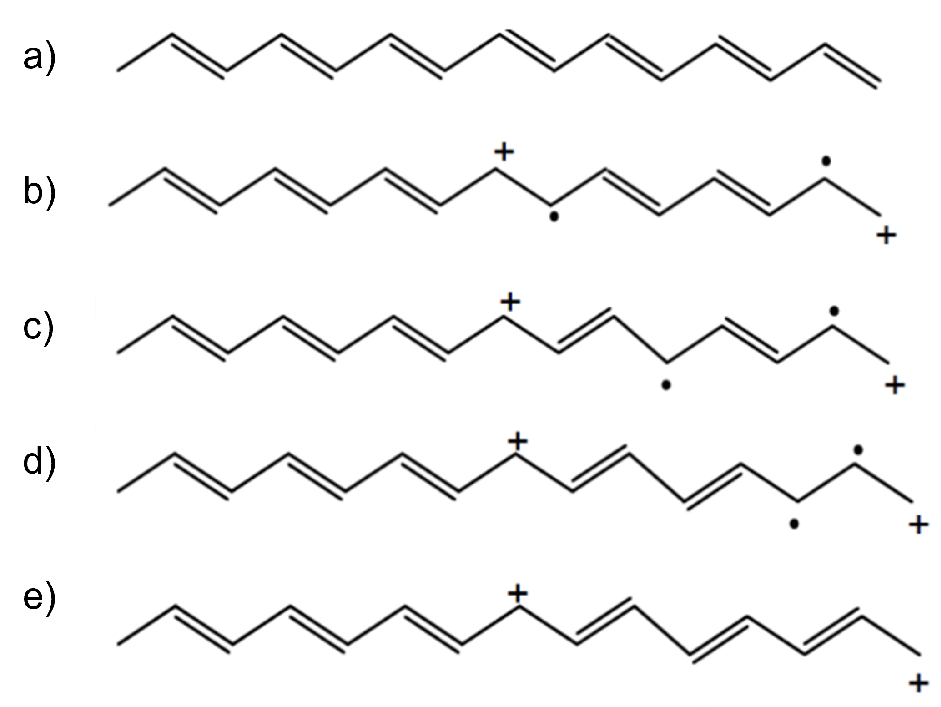
\includegraphics[width=10cm]{Images/pdf/bipolaron.pdf}
  \caption[Representation of bipolaron formation introduced via doping]{a) Structure of degenerate molecule. b) Electron extraction via doping. c) Unpaired electron shifting down. d) Unpaired electrons meet. e) Formation of double bond and two charged polarons: bipolaron.}
  \label{fig:bipol}
\end{figure}

The energy levels generated upon the formation of polarons and bipolarons are represented in Figure \ref{fig:ebipol}. As the doping density increases, the amount of bipolaron states increases as well, the overlapping of them led to the formation of bipolaron bands, and the energy difference between the two in-gap states i and i* decreases (4th image in Figure \ref{fig:ebipol}). %Fix this part % \cite{bredasRoleMobileOrganic1984}
In addition to the new electronic states, the doped polymer will also exhibit distinct optical transitions that could be disclosed by UV-Vis-NIR spectroscopy, although not clearly defined quantitatively \cite{heydarigharahcheshmehTextureNanostructuralEngineering2020}.
%Zozoulenko et al. proposed a new DFT-based description of the polaronic and bipolaronic states 

\begin{figure}[h]
  \centering
  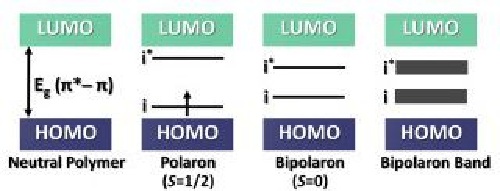
\includegraphics[width=10cm]{Images/pdf/bi-polaron.pdf}
  \caption[Formation of polaron, bipolaron, and bipolaron band]{Potential energy change of aromatic and quinoid in the non-degenerate ground-state neutral conjugated polymer, and formation of polaron, bipolaron, and bipolaron bands upon doping. Extracted from reference \cite{heydarigharahcheshmehTextureNanostructuralEngineering2020}.}
  \label{fig:ebipol}
\end{figure}

%% This specifics introduces to our graph
The use of small molecules is commonly reported as dopants for organic materials. Some strong acceptor (or electron-defficient) molecules that are widely used are 2,3,5,6 tetrafluoro-7,7,8,8-tetracyanoquinodimethane (F$_{4}$TCNQ) or 1,3,4,5,7,8 hexafluoro-7,7,8,8-tetracyanonaphthoquinodimethane (F$_{6}$TCNNQ), which also take part in this work. The latter exhibits a higher electronic affinity (-5.3 eV) or deep HOMO than F$_{4}$TCNQ (-5.2eV) meaning that it can abstract electrons more efficiently, specially from polymers with low ionization potential (less than 5eV) or shallow HOMO \cite{kieferDoubleDopingConjugated2019}%, as it is the case of p(g3T2-T) acting as donor
.

Among the different methods of molecular doping of conjugated polymers, Jacobs et al. compared a solution-mixed and solution sequential doping of P3HT (a thiophene-based polymer) doped with F$_{4}$TCNQ, both straightforward and easy methods for doping. Their work demonstrated that solution-mixed films are considerably rougher than solution-sequential films, affecting negatively its conductivity \cite{jacobsComparisonSolutionmixedSequentially2016}. The fact that solution-sequential doped films possess better homogeneity, make it also more compatible with microstructuring processes such as photolithography. However, this comes at the expense of having less control over the doping levels compared to solution-mixed films \cite{tanOrganicMixedIonic2022}.

\section{Organic Mixed Ionic/Electronic Conductors (OMIECs)} \label{sec:omiecs}

Organic Mixed Ionic/Electronic conductors are organic semiconductors that allow the conduction of electrons (or holes) and ions, the latter set them apart from other organic semiconductors. %Organic semiconductors 
Commonly structured with polar side chains, they have been identified as a promising class of materials for the field of bioelectronics
%These materials, also called organic mixed ionic/electronic conductors (OMIECs), can exchange ions with aqueous electrolytes when electronic charge carriers are injected, transported, and stored in the bulk of the material
\cite{giovannittiEnergeticControlRedoxActive2020}. Initially investigated for batteries and super-capacitors \cite{snookConductingpolymerbasedSupercapacitorDevices2011}
\cite{liangOrganicElectrodeMaterials2012}, where the induction of charges in a semiconducting polymer was the main objective. OMIECs have rapidly grown to include other applications, among them, our focus: OECTs.

Paulsen et al. classified OMIECs into six different categories according to whether they \textit{intrinsically contain ionic charge''} (I, III, V) or not (II, IV, VI), the latter \textit{``contain polar moieties that can solvate ions''}. Another distinction among the categories is whether the conjugated system comprises a single material (homogeneous, type V and VI) or two-component, more complex systems or block co-polymers materials (heterogeneous, type I, II, III, IV)\cite{paulsenOrganicMixedIonic2020}, an schematic representation is shown in Figure \ref{fig:omiectypes}. %For instance, the conjugated polymer p(g3T2-T), used in this work, falls into a type VI OMIEC.s

%Electronic charges accumulated on the conjugated polymer backbone result in secondary property changes in electrochemical potential and electronic conductivity \cite{tanOrganicMixedIonic2022}. 

% PEDOT:PSS Heterogeneous, blends or complexed systems OMIEC. Conjugated polymer/electrolyte blends. Contains ions chemically linked ot an insulating or conjugated component
% p(g3T2-T) Homogeneous, single-component systems OMIEC. Conjugated polymer electrolytes. Ions introduced as free species upon material casting or device operation

%change caption of figure
\begin{figure}[h]
  \centering
  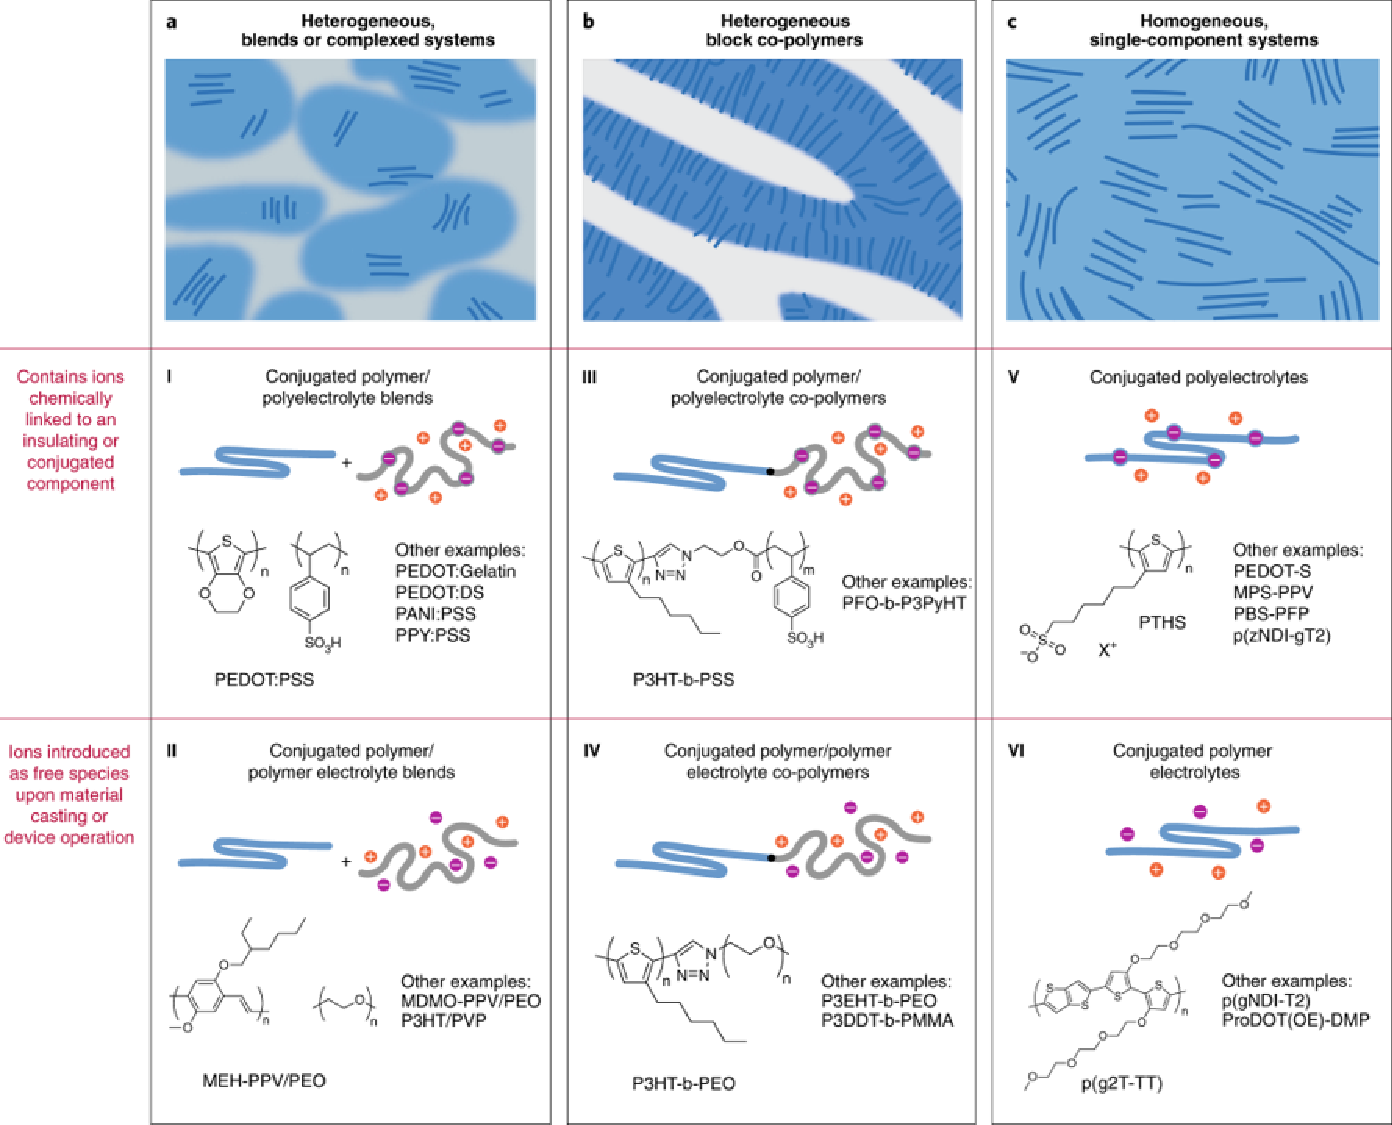
\includegraphics[width=\textwidth]{Images/pdf/OMIEC_types.pdf}
  \caption[Material classes of OMIECs]{\textbf{OMIECs classes.} a) Heterogeneous blends of an conducting conjugated polymer with (I) %an ionic charge bearing
  a polyelectrolyte or (II) an ion-solvating polymer electrolyte. %These systems frequently feature impure phases and can be largely disordered on multiple length scales. 
  b) Heterogeneous block copolymers of a conducting conjugated polymer with (III) %an ionic charge bearing
  a polyelectrolyte or (IV) an ion-solvating polymer electrolyte. %Such block copolymers often feature more well-defined pure phases and mesoscale order—readily synthetically tunable. 
  c) Fully conjugated (V) %ionic charge bearing
  polyelectrolytes and (VI) ion-solvating polymer electrolytes. %OMIEC types I–IV produce heterogeneous morphologies with microphase segregated predominately electron conducting and ion conducting domains. As shown in the sketches in the first row, in the case of blends (I and II) this occurs in a disordered fashion, or in the case of block copolymers (III and IV) it can occur in a variety of ordered structures (lamellar phase portrayed here). All-conjugated polyelectrolytes (V) and polymer electrolytes (VI) exist as a single mixed conducting phase that may contain heterogeneous composition of ordered and amorphous domains. Conceptual sketches (grey, ionic transport component; blue, electronic transport component; orange, cations; magenta, anions) 
  Extracted from reference \cite{paulsenOrganicMixedIonic2020}.}
  \label{fig:omiectypes}
\end{figure}



\subsection{Processes in OMIECs}

\subsubsection{Ionic-electronic interactions}
The presence of electronic charge in OMIECs %remains in
requires also the presence of excess ionic charge, so charge in the system remain balance. In the case of types II, IV and VI OMIECs, the so-called stabilizing electrochemical doping is achieved by the presence of mobile ions, that act as free charges, the remaining type of OMIECs, on the other hand, have this stabilizing charges fixed (chemically bounded). Hence, they are inherently doped.

% Explanation of parts where ion-coupling (electrostatic or direct electron transfer cases) occurs, and a third case where it does not occur, not necessary here, or would it be? I think this is the main difference on what is happening in my material, compared to PEDOT:PSS. So not sure if add the graphs

The amount of coupling between electronic charges and excess ionic charges in OMIECs can be modulated by an applied bias when coupled through an electrolyte \cite{paulsenOrganicMixedIonic2020}. This is the basic principle of OECTs, and it will be further discussed in Section \ref{sec:OECTs}.

\subsubsection{Electronic transport}
%Electronic charge carrier density in undoped semiconductor organic species is logically low (no accessible hopping states), but in contact with an electrolyte, due to the ionic-electronic coupling as described in previous subsection, dopant ions would ... \cite{paulsenOrganicMixedIonic2020}. 

Electronic charge transport mechanisms present in OMIECs are thermally-activated hopping and band-like transport, as represented in Figure \ref{fig:etrans}, which are not different from other conjugated polymers. The former, as its name suggests, is driven by thermal energy and it is limited by the degree of structural disorder, where the weakly-bond electrons in delocalized $\pi$-orbital move along an adjacent $\pi$-orbital within the length of the conjugated polymer, or even between molecules where there is sufficient $\pi$-$\pi$ overlapping. This mechanism is predominant for low electronic charge carrier density and the low density of accessible hopping states. Hopping-like transport results in low mobility and electrical conductivity \cite{paulsenOrganicMixedIonic2020}. 

The band-like transport, on the other hand, occurs normally in OMIECs with increasing doping levels, where the activation energy of charge hopping decreases and carrier mobility increases, leading to diffuse band-like charge transport and it is shown within the polymer-stacking \cite{wangHoppingTransportHall2012}.
%"at extreme doping levels, increased disorder drives carrier localization, which results in a plateau or even decrease in electronic charge carrier mobility"

%"Non-conjugated radical polymers also present a thermally activated mechanism of charge transfer between pendant radical sites, though with a significant dependence on the local self-diffusion of polymer chain to bring radical sites close enough for efficient charge transfer51. This manifests as a hopping transport of electronic carriers (Fig. 2a) that is assisted via segmental motion (described below; Fig. 2g). Also in this case disorder plays a role, producing local variations in the molecular orbital energy levels and spreading orbitals in a density of radical states52."

\begin{figure}[h]
	\centering
	\subfloat[\textbf{Thermally activated hopping}]{{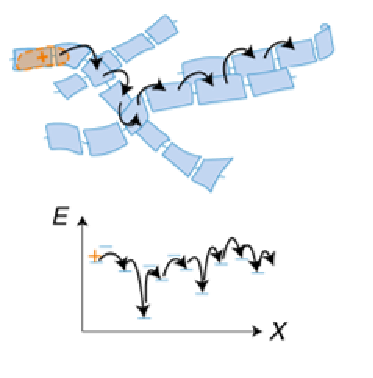
\includegraphics[width=5cm]{Images/pdf/OMIECetransport1.pdf} }}
	%\qquad
	\hspace{2em}
	\subfloat[\textbf{Band-like transport}]{{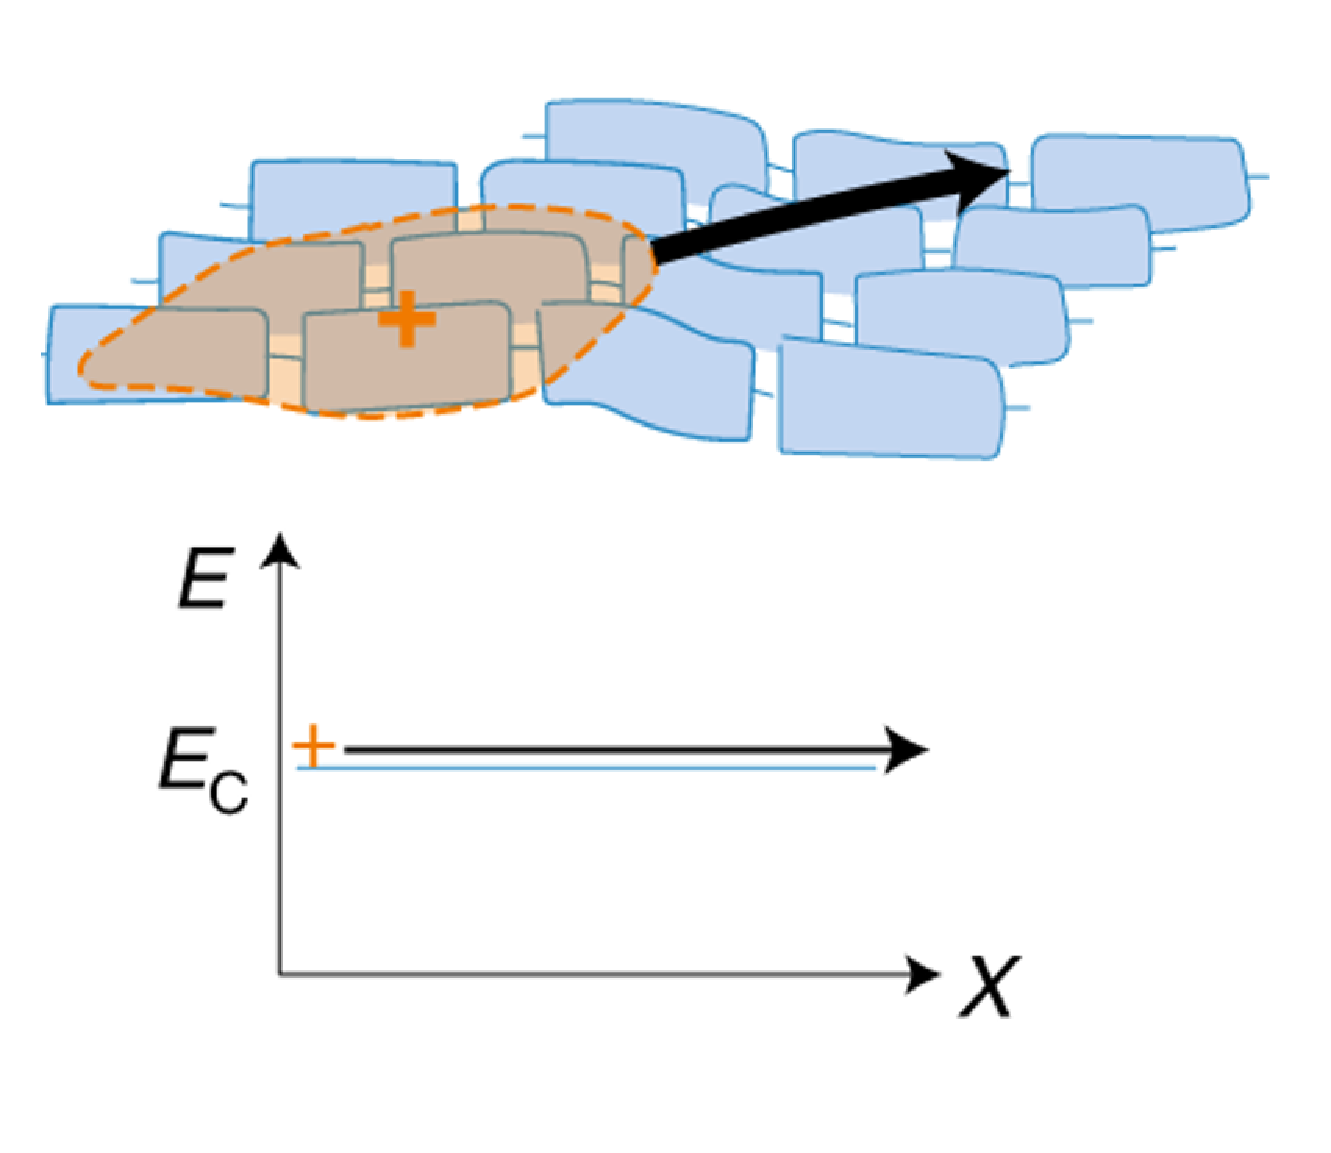
\includegraphics[width=5cm]{Images/pdf/OMIECetransport2.pdf} }}
	\caption[Electronic transport mechanisms in OMIECs]{Schematic representation of electronic charge transport mechanisms: A) Thermally-activated hopping transport %of a relatively localized electronic charge carrier" 
	and B) band-like transport, %of a relatively-delocalized electronic charge carrier"
	where the electronic charge carrier is relatively localized and delocalized, respectively. Extracted from reference \cite{paulsenOrganicMixedIonic2020}.} 
	\label{fig:etrans}
\end{figure}


\subsubsection{Ionic transport}
Although transport of charged anions and cations can be seen in analogy to electrons and holes, it is a more complex process, since ions can be \textit{``multi-valent, and form pairs and larger clusters; morever, they are sensitive to solvent and solvation''} \cite{paulsenOrganicMixedIonic2020}.

Ion transport is unipolar for dry OMIECs of type I, III and V, since they are fixed on a polyelectrolyte, which is not the case for type II, IV and VI, where both anions and cations are mobile. OMIECs in contact with an electrolyte swell, which allows the penetration of excess ions from the electrolyte, therefore both mobile anions and cations would contribute to ion transport to ensure electroneutrality. 

Then two types of ionic charge transport can be differentiated: ion hopping and vehicular solvated-ion transport. In dry or minimally hydrated OMIECs, only ion hopping assisted by segmental motion of the OMIEC side chains or backbone occurs, as shown in Figure \ref{fig:itrans}A; whereas, when the OMIEC is in contact with solvent or liquid electrolyte, both mechanisms are present but predominantly solvated ion vehicle transport. For instance, in water-based electrolytes, proton diffusion occurs via the Grotthuss mechanism, where protons in the water molecules diffuse within the neighboring molecules, this implies a transfer of an ionic effect through the hydrogen-bonded network, as shown in Figure \ref{fig:itrans}B.

Finally, due to the existing ionic-electronic coupling, both ionic and electronic transport in OECTs and other OMIEC-electrolyte based applications, are not independent but are rather complex and needs to consider side effects, such as hydration and electrolyte swelling \cite{paulsenOrganicMixedIonic2020}, which will be further discuss in section \ref{sec:OECTs}.

\begin{figure}[h]
	\centering
	\subfloat[\textbf{Ion hopping} via segmental motion\\\hspace{1em} or ion clusters]{{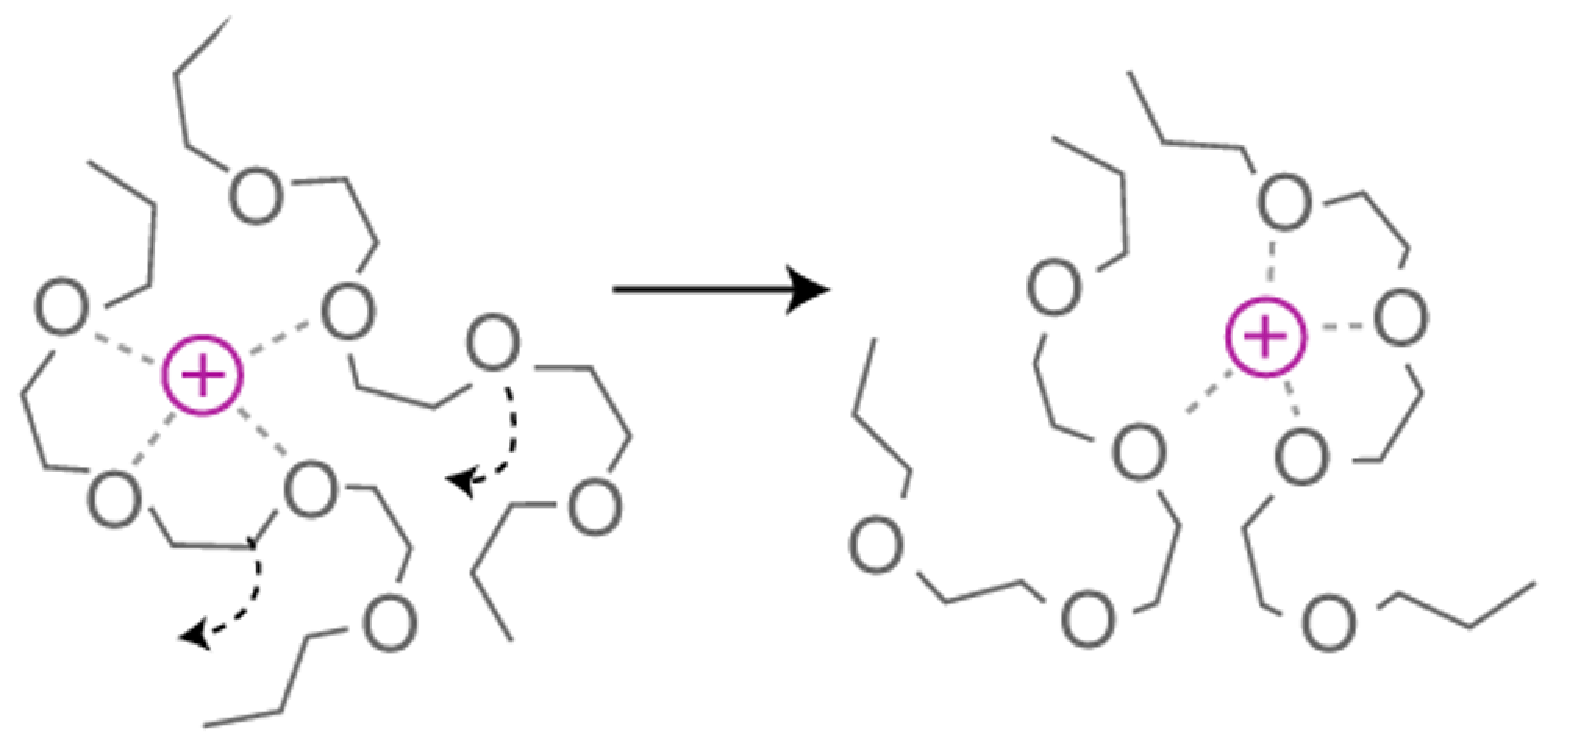
\includegraphics[width=7cm]{Images/pdf/OMIECitransport1.pdf} }}
	%\qquad
	\hspace{2em}
	\subfloat[\textbf{Solvated/vehicle mechanism}]{{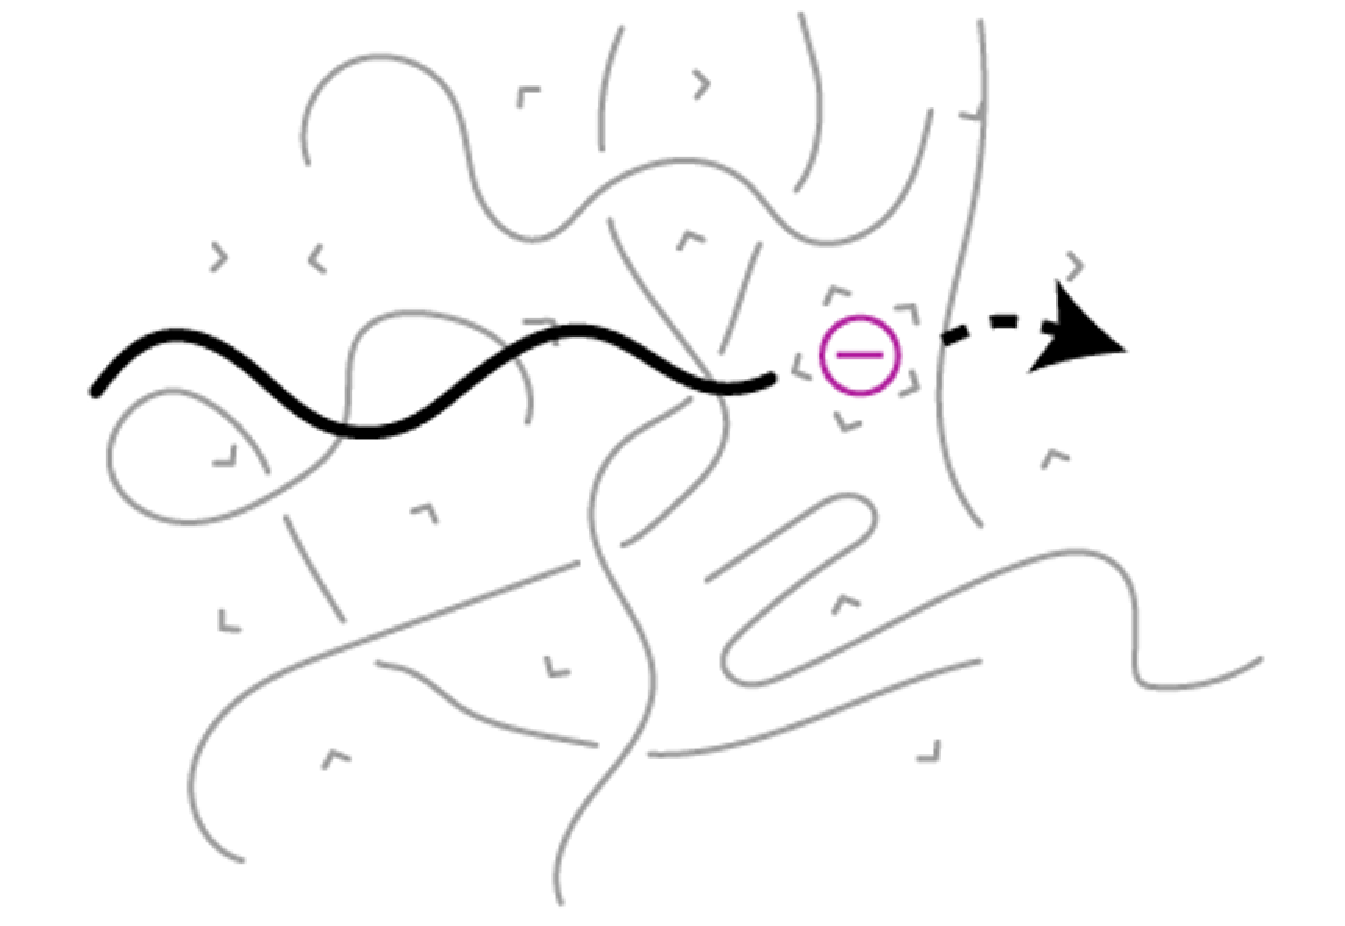
\includegraphics[width=5cm]{Images/pdf/OMIECitransport2.pdf} }}
	\caption[Ionic transport mechanisms in OMIECs]{Schematic representation of ionic charge transport mechanisms: A) Ion hopping via segmented motion and B) vehicular solvated-ion transport. Extracted from reference \cite{paulsenOrganicMixedIonic2020}.}
	\label{fig:itrans}
\end{figure}

%\subsection{Electrochemical Doping}

%As mentioned before, when OMIEC are coupled with an electrolyte and additionally, it is biased with an external gate, ionic-electronic interactions can be modulated. The OMIEC can oxidize or reduce depending on the mobile ions that penetrate the film, ions induced charges allowing its doping.

%Along the morphologic changes of the OMIEC, due to with the generation of permanent distortion in the lattice spacing and expansion in the lamellar direction and contraction in in the $\pi$-$\pi$ direction" \cite{cendraRoleAnionTransport2019}
 
%"The electrochemical charging of OMIECs can be described as a capacitive faradaic charging process,
% there is current caused by charge transfer, other physical phenomenas such as desorption or adsorption can also lead to the aparition of current that is non faradaic reaction
%meaning that the OMIEC" is p-doped (oxidized, in the language of chemists) "through an electron transfer with the contact (current collector), while ions from the electrolyte penetrate inside the channel material to compensate the charge carriers on the polymer backbone electrostatically with no change in the inserted ion's oxidation state" \cite{giovannittiEnergeticControlRedoxActive2020}

%"Electrochemical doping produces a permanent distortion in the lattice spacings, inducing an expansion in the lamellar direction and a contraction in the $\pi$-$\pi$ direction" \cite{cendraRoleAnionTransport2019}

\section{Organic Electrochemical Transistors} \label{sec:OECTs}

Organic Electrochemical Transistors consists of metallic source, drain and gate electrodes, an organic conjugated polymer channel (specifically an OMIEC as described in previous sections) and an electrolyte that couples channel and gate, as represented in Figure \ref{fig:bernard}A. OECTs are devices that have received increasingly attention due to their mechanically compliance, biocompatibility, and are sensitive to biochemical modules \cite{tanMixedIonicElectronic2022}. 

%\begin{figure}[ht]
%	\centering
%	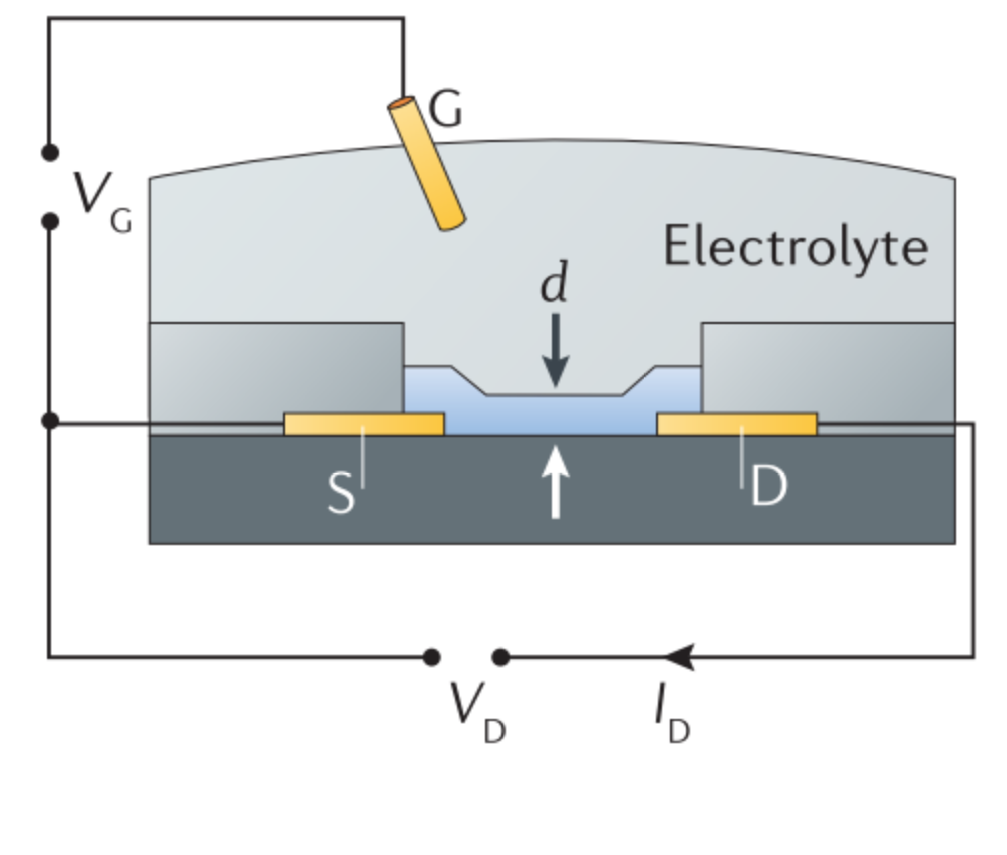
\includegraphics[height=4.5cm]{Images/structure.png}
%	\caption{Typical structure of an organic electrochemical transistor (OECT) \cite{rivnayOrganicElectrochemicalTransistors2018}.}
%	\label{fig:modes}
%\end{figure}


\subsection{Device Physics} \label{subsec:devphy}

Although the structure of OECTs is different from conventional metal-oxide-semiconductor field-effect transistors (MOSFETs), the basic understanding of the latter can give us a clear idea of how OECTs operate. Unlike MOSFETs, OECTs are coupled with an electrolyte rather than an insulator, as seen in Figure \ref{fig:vsMOS}. So, when applying a gate voltage, instead of polarizing the dipoles in the insulator, creating a field that causes accumulation of carriers at the interface of the semiconductor/insulator as it happens in a MOSFET, in an OECT, the gate voltage drives ions to penetrate the bulk of the channel, therefore accumulation of carriers will happen throughout the whole volume of the OMIEC film. This mechanism explains the large gate-channel capacitance in these devices compared to MOSFETs, and why the drain current takes into account a volumetric capacitance \cite{friedleinDevicePhysicsOrganic2018}.


\begin{figure}[h]
  \centering
  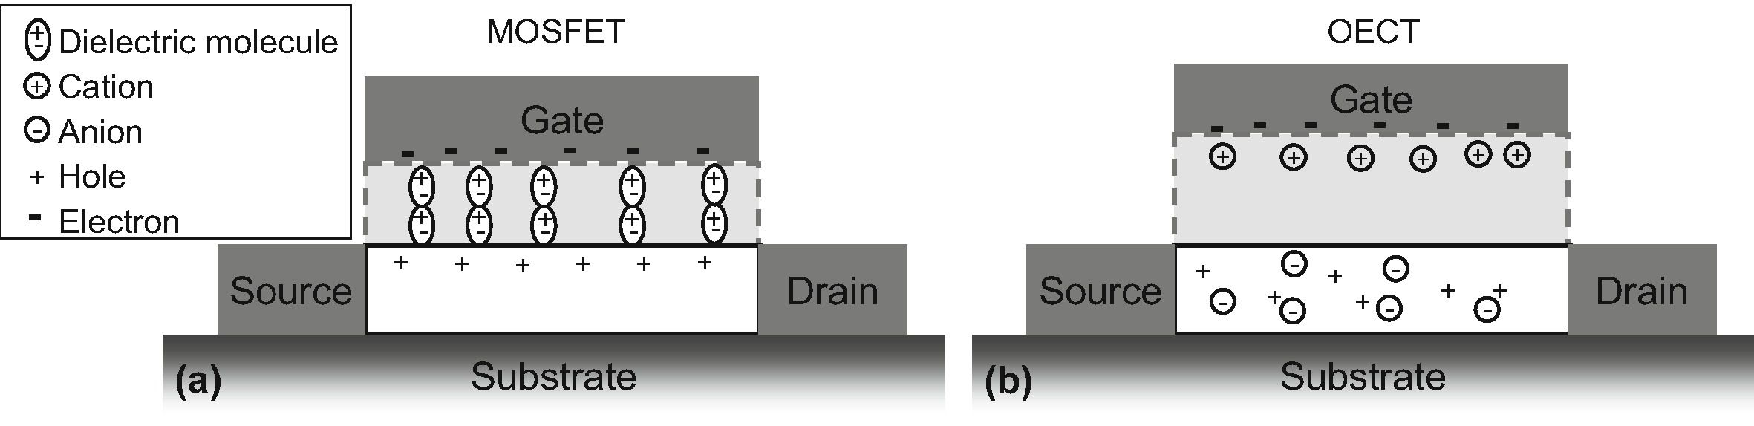
\includegraphics[width=\textwidth]{Images/pdf/MOSFETvsOECTs.pdf}
  \caption[Device physics of MOSFET vs OECT]{Comparison of p-type A) MOSFET and B) OECT, where the light-gray region represents an insulator and a electrolyte, respectively. Extracted from reference  \cite{friedleinDevicePhysicsOrganic2018}}
  \label{fig:vsMOS}
\end{figure}

Bernards and Malliaras implemented a model based on a p-type depletion-mode OECT (based on PEDOT:PSS since it is widely fabricated and investigated, further discussion in the following section). The model divides the behavior of the OECT into an electronic (source-channel-gate structure) and an ionic circuit (gate-electrolyte-channel structure). The electronic circuit is treated as a \textit{variable} resistor therefore it is modeled using Ohm's law. Its variability lies on the fact that upon the application of a positive gate voltage, de-doping of the semiconductor occurs, analogous to the compensation doping of silicon, cations from the electrolyte penetrate the polymer, compensating one acceptor. Meanwhile, the ionic circuit consists of a resistor that represents the flow of ions in the electrolyte, in series with a capacitor, representing the storage of ions in the channel as shown in Figure \ref{fig:bernard}B  \cite{rivnayOrganicElectrochemicalTransistors2018}\cite{bernardsSteadyStateTransientBehavior2007}. 

\begin{figure}[h]
	\centering
	\subfloat[Typical OECT structure]{{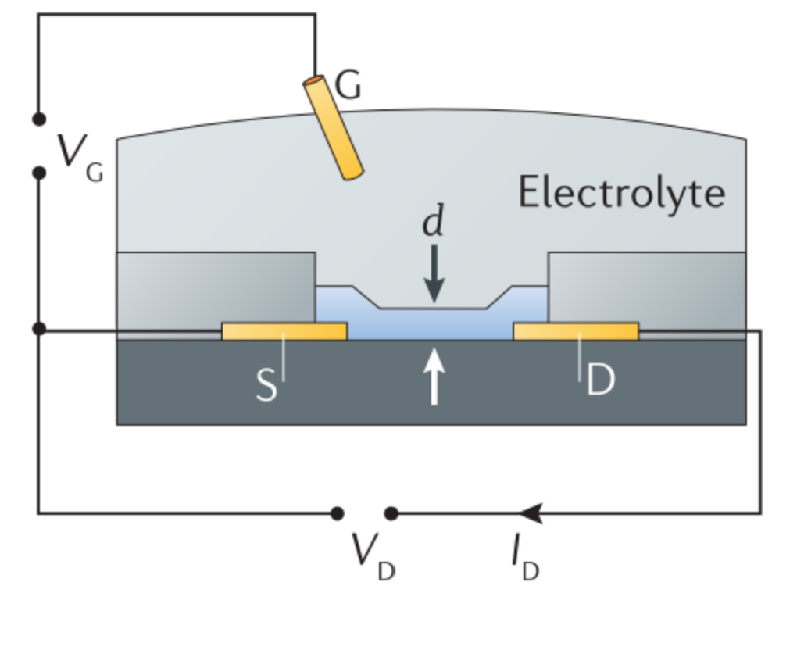
\includegraphics[width=3.5cm]{Images/pdf/structure.pdf} }}
	%\qquad
	%\subfloat[]{{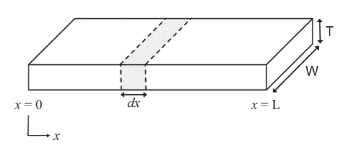
\includegraphics[height=1.5cm]{Images/film_model.png} }}
	%\subfloat[]{{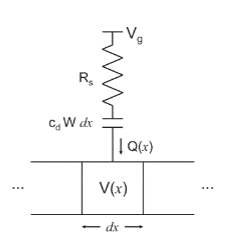
\includegraphics[height=4.5cm]{Images/circuit_model.png} }}
	\hspace{2em}
	\subfloat[Electronic and ionic circuits]{{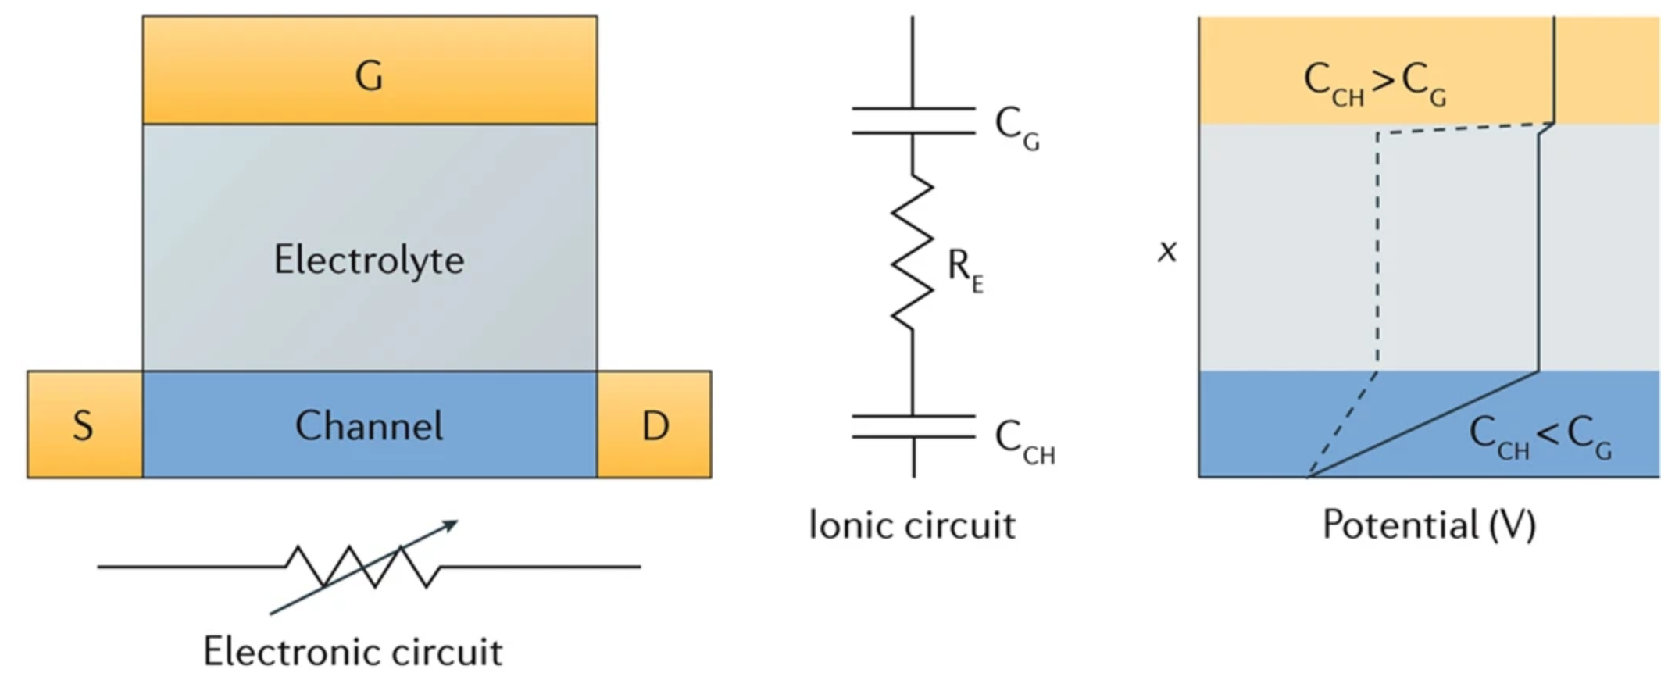
\includegraphics[width=8cm]{Images/pdf/circuits.pdf} }}
	\caption[Typical OECT structure and circuit model]{A) Typical structure of an organic electrochemical transistor (OECT). B) (Left) Electronic circuit modelled as a resistor with a varible resistance. (Right) Ionic circuit consisting of channel (C$_{CH}$) and gate (C$_{G}$) capacitors, coupled with a resistor corresponding to the electrolyte (R$_{E}$). Extracted from reference \cite{rivnayOrganicElectrochemicalTransistors2018}.}
	\label{fig:bernard}
\end{figure}


\subsection{Operation Modes}

Analogous to conventional MOSFETs, depending on whether the device needs a gate potential to turn it ON, it will describe two operation modes: depletion and enhancement (the latter commonly named as accumulation for OECTs). These operation modes have a strict relationship to the channel material%, if it is inherently conductive or semiconducting
.

\begin{figure}[h]
	\centering
	\subfloat[Depletion-mode OECT]{{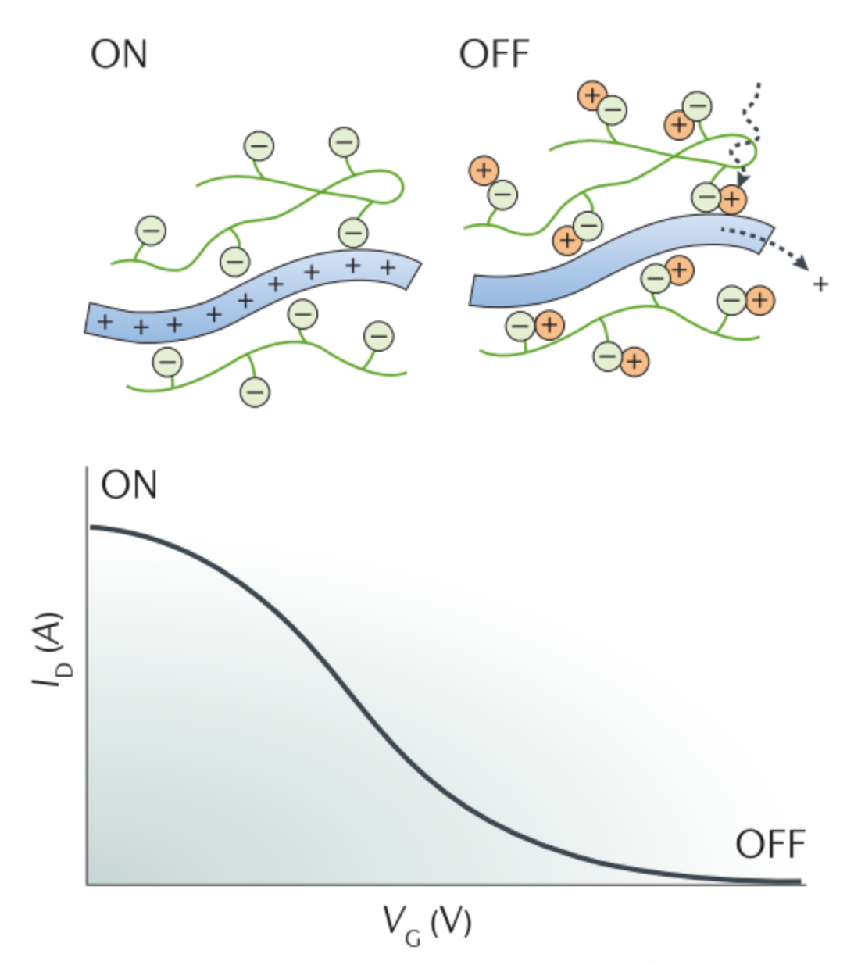
\includegraphics[height=7cm]{Images/pdf/depletion.pdf} }}
	\hspace{2em}
	\subfloat[Accumulation-mode OECT]{{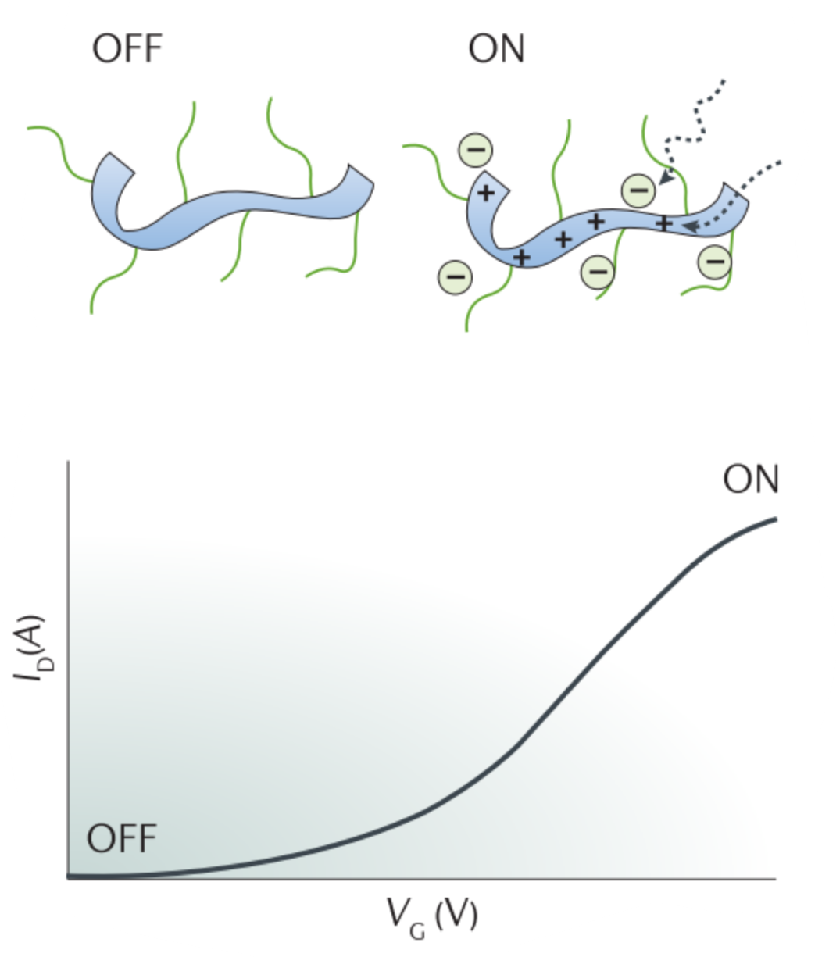
\includegraphics[height=7cm]{Images/pdf/accumulation.pdf} }}
	\caption[Depletion- and accumulation-mode OECTs]{(A) Transfer curve showing depletion-mode operation of a p-type OECT with a conducting polymer channel. (B) Transfer curve showing accumulation-mode operation of a p-type OECT with a semiconducting polymer channel. Images extracted from reference \cite{rivnayOrganicElectrochemicalTransistors2018}.}
	\label{fig:modes}
\end{figure}

As seen in Figure \ref{fig:modes}A) and B), the polymer can be intrinsically doped (conductive) or undoped (insulating). In the first scenario, the OMIEC already possesses anions which have had induced charges within its backbone, therefore it needs the injection of cations to counteract this effect, hence turn off the device. The opposite scenario is presented for an insulating polymer channel, a zero-gate biased OECT would have no charges in its backbone hence the device will be in OFF state, it will need the application of a gate voltage to drive anions into the polymer and induce charges.

\subsubsection{Standard material for depletion-mode OECTs}

Poly(3,4-ethylenedioxythiophene) poly(styrene-sulfonate) (PEDOT:PSS) is a \textit{``degenerately doped''} \cite{bernardsSteadyStateTransientBehavior2007} or conductive polymer that is widely used in multiple applications in organic electronics. Classified as type I OMIEC, as seen in Figure \ref{fig:omiectypes}, it is a blend between a conjugated polymer (PEDOT) and a polyelectrolyte (PSS), the latter possesses chemically linked ions and serves as a polymeric acid template to allow dispersable suspensions \cite{paulsenOrganicMixedIonic2020}.

Due to its commercial availability, operational stability, and relatively high performance, PEDOT:PSS became a standard material for p-type OECTs. Its main drawback lays in its depletion-mode operation, since, as explained in the previous section, requires power to turn off. 

With the aim of minimizing power consumption, there is a special interest to fabricate accumulation-mode devices with high performance \cite{nielsenMolecularDesignSemiconducting2016}\cite{tanOrganicMixedIonic2022}\cite{inalBenchmarkingOrganicMixed2017}\cite{keeneEnhancementModePEDOTPSS2020}. This type of devices have the advantage of dissipating less static power when the device is not operated, due to low OFF current %, which must be minimized as much as possible
\cite{giovannittiEnergeticControlRedoxActive2020}.

\subsubsection{Prospective materials for accumulation-mode OECTs}
% As a widely studied material, 
PEDOT:PSS was not descarted as a possible accumulation-mode OECT, Keene et al. used a series of amines to de-dope PEDOT:PSS and obtain OECTs with negative turn-on voltages \cite{keeneEnhancementModePEDOTPSS2020}. However, synthetically modifying PEDOT:PSS in a controlled manner remains complicated. Parallel to these efforts, the design of new semiconducting polymers with the aim of not only having acummulation-mode OECTs but enhancing performance is also studied. Nielsen et al. reported a series of semiconducting polymers with Triethylene glycol (TEG) side chains with good performance. Among the five thiophene- and benzodithiophene-based polymers, they found out that the %TEGylated 
backbone consisted of 2,2'-bithiophene polymerized with other thiophene molecule (g2T-T), as seen in Figure \ref{fig:g2TT}, showing the highest performance %, even higher transconductance over PEDOT:PSS
\cite{nielsenMolecularDesignSemiconducting2016}.

\begin{figure}[h]
	\centering
	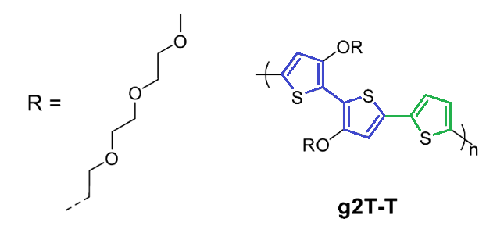
\includegraphics[width=7cm]{Images/pdf/g2T-T.pdf}
	\caption[Chemical structure of polymer g2T-T]{Chemical structure of polymer with backbone g2T-T, R representing the side chain. Extracted from reference \cite{nielsenMolecularDesignSemiconducting2016}}
	\label{fig:g2TT}
\end{figure}

Moser et al. took the same backbone and studied the impact of the length of the ethylene glycol (EG) side chain on the performance of OECTs. They reported that reducing chain length maximized both the capacitance and mobility; nonetheless, it was unfavorable for ion-polymer interaction. Finally, they suggested an optimum-side-chain length of 3 monomers (over 2, 4 and 6 monomers), demonstrating that an OECT with 3-(2-(2-(2-methoxyethoxy)ethoxy)ethoxy)thiophene (p(g3T2-T)) has a turn-on voltage close to zero and better performance compared to other thiophene-based species (as seen in Figure \ref{fig:pg3t}), even better than PEDOT:PSS OECTs %. This advantage does not remain the only one, since p(g3T2-T)  would not require extensive pre- and postprocessing to optimize stability and electrochemical performance in aqueous media as PEDOT:PSS
%% actually the last part came from references 14-16 of that papers.
\cite{moserEthyleneGlycolBasedSide2020}.

\begin{figure}[h]
	\centering
	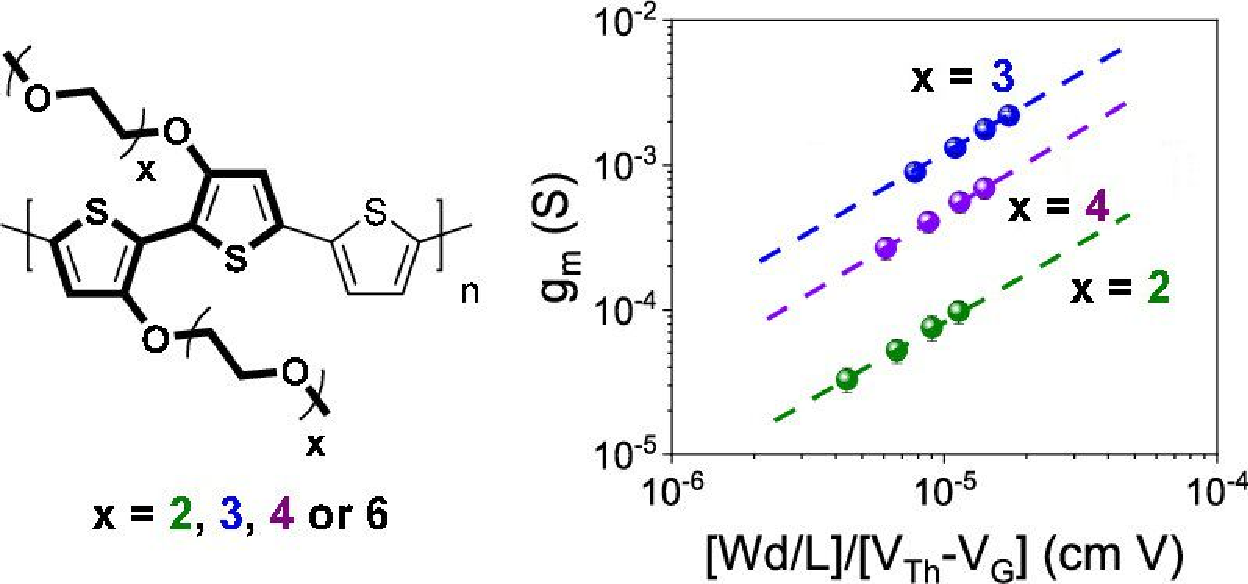
\includegraphics[width=10cm]{Images/pdf/pg3t+perf.pdf}
	\caption[Chemical structure and transconductance of g2T-T with side-chain engineering]{(Left) Chemical structure of the repeat units for p(gxT2-T). (Right) Transconductance vs channel geometry and operating parameters of p(gxT2-T) for x = 2, 3 and 4. Extracted from reference \cite{moserEthyleneGlycolBasedSide2020}.}
	\label{fig:pg3t}
\end{figure}

The structural tuning of this polymer was thought to have a backbone that warrants reversibility during electrochemical redox reactions and good electronic transport, meanwhile having side chains that enable its stability in aqueous electrolytes and efficient transport of ionic and electronic charge carrier \cite{moiaDesignEvaluationConjugated2019}. 
%% moia es el unico que tiene un dibujo distinto de pg3t
%Additionally, , and the absence of extensive pre- and postprocessing to optimize polymer stability and electrochemical performance in aqueous media %and the possibility of an accumulation-mode OECT with low operation voltages put it on top of compared to PEDOT:PSS \cite{moserEthyleneGlycolBasedSide2020}.

%Seria chevere tener un grafico de como thiophene publications empezaron a crecer.
%Thiophene is a planar conjugated ring structure consists of six delocalized pi-electrons. The aromatic nature arises from the four $\pi$-electrons and one unshared lone pair of electrons of the oxygen as six delocalized $\pi$-electrons. It folow Hucke´s rule. Hence it is aromatic compound.

%Homogeneous single phase OMIECs (types V and VI) display larger magnitudes of ionic–electronic coupling and larger values of volumetric capacitance than biphasic OMIECs (types I–IV) \cite{paulsenOrganicMixedIonic2020}. 

Under the classification shown in Figure \ref{fig:omiectypes}, p(g3T2-T) can be identified as a type VI OMIEC that comprises a conjugated polymer with ions introduced as \textbf{free species} wheareas PEDOT:PSS' ions are \textbf{chemically linked} to the polyelectrode (PSS). This structural characteristic make p(g3T2-T) display larger magnitudes of ionic-electronic coupling and volumetric capacitance than biphasic OMIECs (such as PEDOT:PSS) \cite{paulsenOrganicMixedIonic2020} and at the same time will be important for understanding the challenges on having a stable OECT, further discussion in Section \ref{subsec:sidereac}.
%% Replace further discussion for a table with numbers of the two polymers

\subsection{Important Figures of Merit}

\subsubsection{Transconductance}
Transconductance is considered as the most important parameter to measure any transistor's amplification capability, calculated as the first-order derivative of the output current (drain current) with respect to the input voltage (gate-source voltage): $g_{m} = \sfrac{\partial I_{D}}{\partial V_{GS}}$. Bernards and Malliaras calculated this parameter from their implementation of a mathematical model for depletion-mode p-type OECTs \cite{bernardsSteadyStateTransientBehavior2007}, as previously seen in Section \ref{subsec:devphy}. Including also n-type, the following equation expresses the transconductance: %\ref{eq:gm}:

\begin{equation}\label{eq:gm}
	g_{m} = \frac{Wd}{L} \mu C^{*} |(V_{th} - V_{G})|,
\end{equation}

where $W$, $L$ and $d$ are the channel width, length and thickness, respectively, $\mu$C* product, the gate voltage ($V_{G}$) and threshold voltage ($V_{th}$), which will be discussed in the next subsections.

Commonly, the maximum value of transconductance is reported ($g_{m,max}$), which falls into the saturation regime. Inal et al. reported the maximum transconductance of various channel materials at different device geometry parameters using a Ag/AgCl pellet as reference/gate electrode and 0.1M NaCl as electrolyte, showing OECTs with polymerized-g2T-backbones, the best performances, within the range of 1 to 30 mS, depending on the geometry (Figure \ref{fig:gmuc}A) \cite{inalBenchmarkingOrganicMixed2017}.

\subsubsection{$\mu$C* product}

$\mu$C* is the most important parameter for benchmarking OECT channel materials, that represents both ionic and electronic transport properties %storage ability
\cite{inalBenchmarkingOrganicMixed2017}. %\cite{inalHighTransconductanceAccumulation2014}. %% Other accumulation mode OECT with PTHS
It is the product of two important parameters, $\mu$, the electronic mobility, and C*, the volumetric capacitance, the latter encloses the ion penetration, transport, and storage ability of the OMIEC film.

Along with the transconductance, Inal et al. extracted the values of $\mu$C* from the calculating the linear slope of the maximum transconductance and channel geometry (Figure \ref{fig:gmuc}A), following Equation \ref{eq:gm}. She correlated her results with the independent calculation of both parameters, showing again polymerized-g2T-backbones with the highest value of 261 $\pm$ 29 $Fcm^{-1}V^{-1}s^{-1}$,   and among the materials that have closest 1:1 relation for both methods of calculation the $\mu$C* product (Figure \ref{fig:gmuc}B) \cite{inalBenchmarkingOrganicMixed2017}.
 
 \begin{figure}[h]
 	\centering
 	\subfloat[]{{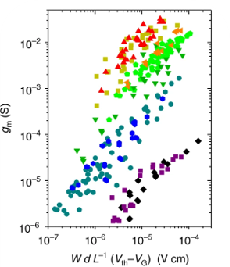
\includegraphics[width=4.5cm]{Images/pdf/gm_sizes.pdf} }}
 	\hspace{2em}
 	\subfloat[]{{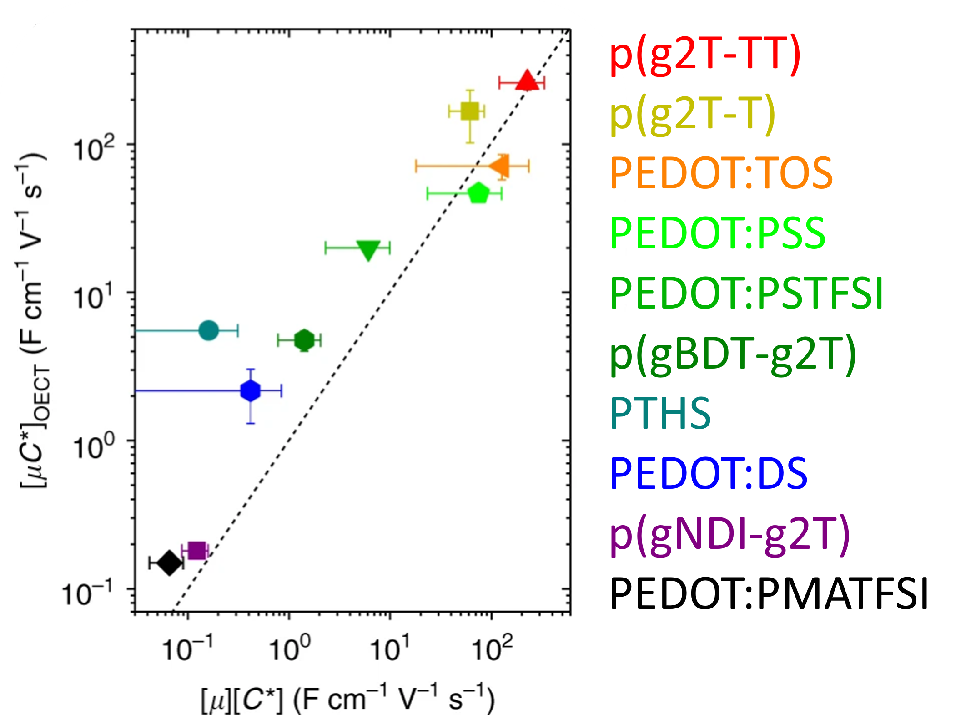
\includegraphics[width=7cm]{Images/pdf/uc_omiecs.pdf} }}
 	\caption[OECTs benchmark with different OMIECs]{A) Plot of $\mu$C* product calculated by the linear slope between transconductance and channel geometry. B) Calculated slope from A) in function of the product of independent determination of $\mu$ and C*, dotted line representes the 1:1 relation between both methods of calculation. Extracted from reference %\cite{ohayonSaltsAdditivesRoute2023} 
 		\cite{inalBenchmarkingOrganicMixed2017}.}
 	\label{fig:gmuc}
 \end{figure}

The independent calculation of $\mu$ is yet difficult due to the presence of ionic species, normally calculated in transient regimes, taking advantage of ions' lower mobility, which is out of the scope of this work. Among the method to calculate C*, performing Electrochemical Impedance Spectroscopy (EIS) is a straightforward one, and by using Equation \ref{eq:C} to calculate the capacitance, at low frequency ranges where the capacitance should describe a plateau, since the modulation of AC is slow enough to fully populate the OMIEC with ions. Finally, the value is divided the calculated capacitance by the film volume to obtain C*%. Another approach is to use cyclic voltammetry (CV)
 \cite{ohayonGuideCharacterizationOrganic2023}.

\begin{equation} \label{eq:C}
	C = \frac{1}{2\pi \cdot f \cdot |Z^{img}|},
\end{equation}
where $Z^{img} (\Omega)$ is the imaginary part of the impedance and $f$ is the frequency (Hz).

The calculation of this capacitance is under a fixed-gate biased condition, it is important to remember that the modulation of the degree of electrochemical doping in OECTs with an applied biased, will manifest a potential-dependent capacitance (C)%. Homogeneous single phase OMIECs (type V and VI) display larger magnitudes of ionic-electronic coupling and larger values of volumetric capacitance than biphasic OMIECs such as PEDOT:PSS 
\cite{inalBenchmarkingOrganicMixed2017}.
% found in Paulsen \cite{paulsenOrganicMixedIonic2020}
%actually from reference 44, benchmarking omiecs for transistors

\subsubsection{Threshold voltage}

From the steady-state characteristics of an OECT, specifically the transfer characteristics ($I_{D}$ vs $V_{GS}$), one can calculate not only the transconductance but also the ON/OFF ratio and the threshold voltage ($V_{th}$). The latter can be determined by plotting the square root of $I_{D}$ as a function of $V_{GS}$ and extrapolate the linear portion of the slope, where the intersection with the x-axis will give this parameter \cite{ohayonGuideCharacterizationOrganic2023}.

In OECTs, it represents the \textit{``film's readiness for ion penetration''} \cite{ohayonGuideCharacterizationOrganic2023}. Controlling and/or shifting this parameter is wished, specially to integrate transistors and meet any circuit requirement and control operation, noise margins, and power consumption. 

 \begin{figure}[h]
	\centering
	\subfloat[]{{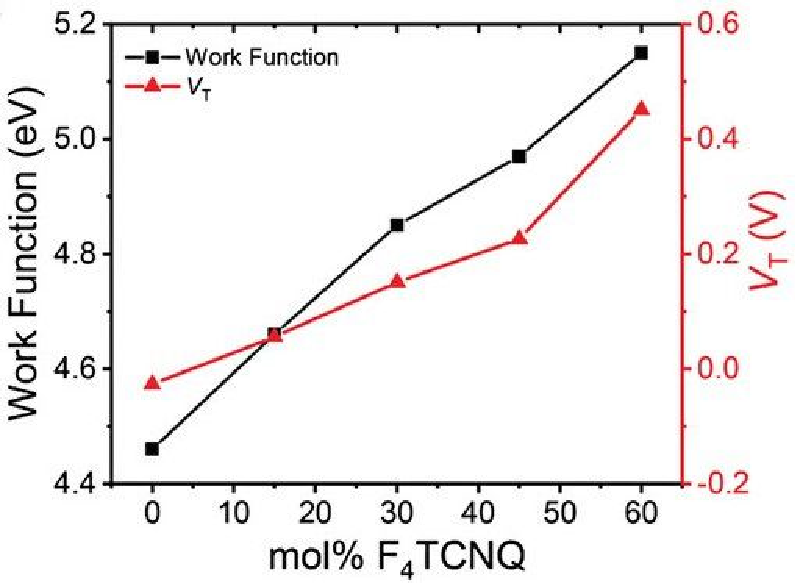
\includegraphics[width=5.8cm]{Images/pdf/wf_shift.pdf} }}
	\hspace{2em}
	\subfloat[]{{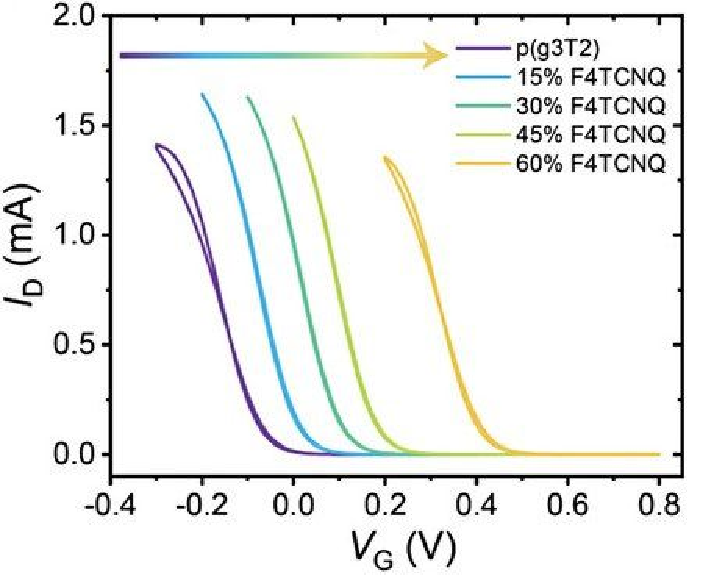
\includegraphics[width=5cm]{Images/pdf/vth_shift.pdf} }}
	\caption[Tuning of threshold voltage with different levels of doping p(g3T2-T)]{Controlling OECT threshold voltage by chemical doping of p(g3T2-T) gate electrode with F$_{4}$TCNQ. A) Plot of threshold voltage and gate work function for doped gates of different dopant concentrations. B) Transfer curves of p(g3T2-T) channel OECT %(L = 10 µm; W = 2000 µm; VD = −0.1 V, VG scan rate of 20 mV s−1) 
		with p(g3T2) gates of various F$_{4}$TCNQ dopant concentrations. . Extracted from reference \cite{tanTuningOrganicElectrochemical2022}.}
	\label{fig:tune}
\end{figure}

The chemically de-doping of PEDOT:PSS by Keene et al. described in previous sections, is also an approach to shift the threshold voltage, until reaching negative values, characteristic for accumulation-mode OECTs \cite{keeneEnhancementModePEDOTPSS2020}. Tan et al., on the other hand, explored a different approach, rather than modifying the doping level of the channel, they tuned the doping level of the gate to shift the threshold voltage. They used p(g3T2-T) and obtained a 400mV change with 60\% mol ratio of 2,3,5,6-Tetrafluoro-7,7,8,8-tetracyanoquinodimethane (F4TCNQ) dopant, as seen in Figure \ref{fig:tune}. The advantage over this approach is i) protecting the material from oxidation with air, since the Fermi level in brought towards the highest occupied molecular orbital (HOMO), and ii) no interference with the channel which helps to leave the transconductance unaffected \cite{tanTuningOrganicElectrochemical2022}.


\subsection{Side Reactions} \label{subsec:sidereac}

%Achieving effective charge transfer between the analyte and OMIEC requires appropriate alignment of the electrochemical potential of electrons on the OMIEC electrode and the redox specie. Failure to do so may result in the subsequent transfer of charges to other redox-active sinks in the environment, leading to undesirable side reactions and products that may interfere with the OMIEC’s operation. Electrons flow from a region of higher to lower electrochemical potential. Hence, achieving electron transfer from redox-active species to the OMIEC requires the latter to have a deep LUMO (high electron affinity) \cite{tanMixedIonicElectronic2022} %paper

%Capacitive fading upon cycling

\subsubsection{Water uptake and swelling}

%Although there are some studies in non-water-based electrolytes, such as ionic liquids. 
Water-based electrolytes are widely used, and even in the pursue of solid-state OECTs, precursors have a certain degree of water content \cite{weissbachPhotopatternableSolidElectrolyte2022}\cite{nguyen-dangBiomaterialBasedSolidElectrolyteOrganic2021}, hence, side reactions of OMIECs upon water contact are inevitable and therefore, studies to understand the impact are necessary.  %and some bioelectronics applications will inevitable operate under water environment, 
Water uptake in OMIECs cause their increase of mass (swelling) and change in morphology. Water uptake happens since OMIECs will need to compensate their intrinsic doping. Therefore, \textit{``the effect of doping-induced hydration on the OMIEC morphology must be taken into account when designing OECTs''} \cite{savvaBalancingIonicElectronic2020}.

Savva et al. studied the influence of water on the performance of PEDOT:PSS OECT, the water uptake %of conjugated polymer films 
led to 10-13\% mass increase under non-biased conditions. As the concentration of water decreased (NaCl$_{aq}$ 10 mM, 100mM, 1M, and 6M) ionic charging got faster; %regardless of the doping pulse, 
however, the fastest %ionic charging 
response time is not achieved by the highest salt concentration but rather NaCl$_{aq}$ 1 M. This due to attractive forces between counter ions which % the injection/drift of ions is also affected by the ion-counterion, attractive forces in NaCl$_{aq}$ 6 M 
hinders the drift of anions, hence delays the ion injection from the electrolyte %, opposing their drift into the polymer affecting the response time. %Water irreversibly changes the film morphology, In general, while ion transport is enhanced, electronic charge transport is negatively impacted 
\cite{savvaInfluenceWaterPerformance2019}.

%Swelling is produced due to the compensation doping in the film, the ratio of swelling is normally reported and calculating by measuring the length of  by estimating "the number of electrolyte ions compensating for the electronic charge carriers" in the OMIEC. \cite{ohayonGuideCharacterizationOrganic2023}. %Savva et al. demonstrated that polymers in contact with water and are used for enhancement mode OECTs detriment its electronic charge transport, since water irreversibly changes the film morphology, but at the same time enhances ion transport \cite{savvaInfluenceWaterPerformance2019}

%\subsubsection{Water uptake}
In another study, Savva et al. showed that a certain level of hydration is necessary for facile ionic transport, but can negatively impact electronic charge transport, in glycol-based side chains \cite{savvaBalancingIonicElectronic2020}, commonly used in accumulation-mode OECTs and where ionic transport is already enhanced by side-chain engineering \cite{moiaDesignEvaluationConjugated2019}. %increased its transconductance by five orders of magnitude, due to an increase in C* and charge carrier mobility. %\cite{siemons}


\subsubsection{Oxygen Reduction Reaction (ORR)}

Oxygen Reduction Reaction is a common undesirable side reaction at environmental conditions, specially among devices fabricated with polymers with low ionization potential (IPs). The utilization of OMIECs with low IP are frequent in accumulation-mode OECTs. 


%With the aim of developing accumulation-mode OECTs, the engineering of new OMIECs were introduced as commented in previous sections. Normally, this polymer backbones have low ionization potential (IPs) which lead to another side effect issue that little attention has been paid: non capacitive faradaic rections in ambient: electron-transfer reaction from the OMIEC to molecular oxygen described as oxygen reduction reaction (ORR)

% Remember 
% Thermodynamically favored processes or reactions are those that involve both a decrease in the internal energy of the components (ΔH° < 0) and an increase in entropy of the components (ΔS° > 0). These processes are necessarily “thermodynamically favored” (ΔG° < 0) or negative. ΔG° = ΔH°-TΔS°
% Catalyst help to reduce the activation energy required for a reaction
The ORR is a non-capacitive faradaic reaction between the OMIEC and molecular oxygen, where electron-transfer occurs. The reaction yields either hydrogen peroxide (H$_{2}$O$_{2}$) or water (H$_{2}$O), as described in \ref{eq:h2o2} and \ref{eq:h2o}, or oxidation (p-doping) of the OMIEC that acts as the catalyst \cite{giovannittiEnergeticControlRedoxActive2020}. 

%The first shows a free energy difference that is endergonic for OMIECs with IPs > 4.9eV and hence prevent the OMIEC from undergoing ORR that form H$_{2}$O$_{2}$. To prevent the ORR in ambient conditions, OMIECs based on donor-acceptor copolymer (Type III or IV) that have large IPs to shift

% Actually this material does not avoid this, we need to take into account this interaction.


\begin{equation}\label{eq:h2o2}
	{E^{0}}_{O_{2}/H_{2}O_{2}} : O_{2} + 2H^{+} + 2e^{-} \rightarrow H_{2}O_{2}
\end{equation}

\begin{equation}\label{eq:h2o}
	{E^{0}}_{O_{2}/H_{2}O} : O_{2} + 4H^{+} + 4e^{-} \rightarrow 2H_{2}O
\end{equation}

As seen in Figure \ref{fig:orr}, $\eta_{1}$ and $\eta_{2}$ represent free energy difference between reactants and the reaction products H$_{2}$O$_{2}$ and H$_{2}$O, respectively. If this free energy is negative, the reaction is endergonic (the opposite is exergonic), and needs energy to be driven. PEDOT:PSS and p(g3T2-T) exhibit exergonic reactions. For instance, a polymer with higher IP (> 4.9eV) would be needed to prevent oxygen peroxide to form.

\newpage
\begin{figure}[!ht]
	\centering
	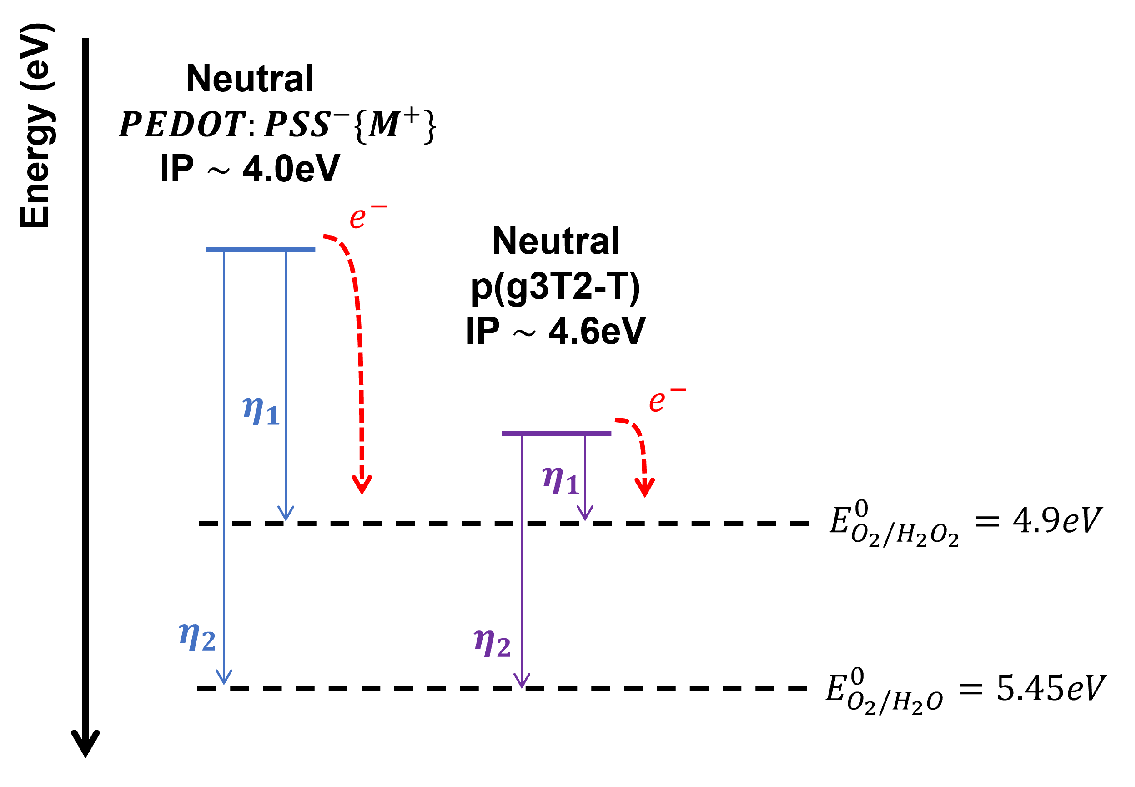
\includegraphics[width=10cm]{Images/pdf/ORR.pdf}
	\caption[Energy levels of neutral state of OMIECs related to oxygen reduction reactions potentials]{Simplified mechanism of two- and four-electron Oxygen Reduction Reactions with neutral states of OMIECs: p(g3T2-T) and PEDOT:PSS. The free energy difference between reactant and the reaction products is represented by $\eta$. Image adapted from reference \cite{giovannittiEnergeticControlRedoxActive2020}, where values are defined from cyclic voltammetry measurements using Ag/AgCl as reference electrode and NaCl as electrolyte.}
	\label{fig:orr}
\end{figure}

%\subsection{Photo-patternable Solid-State OECTs}

%\subsection{Building Block for neuromorphic and bioelectronic applications}


%%% Local Variables: 
%%% mode: latex
%%% TeX-master: "thesis"
%%% End: 
